
%----------------------------------------------------------------------------------------
% Mini page taking up 66% of the actual page
\begin{minipage}[t]{\dimexpr0.5\linewidth-1em}

\begin{figure}[H]
\centering
\includegraphics[width=0.4\linewidth]{figure/logo-aka.jpg}
\end{figure}

\textbf{Aikikai NSW Attendance System, 8th Nov 2020.}

Aikikai NSW is trialing a new web based attendance tracking system.
This new system will help us maintain more accurate records,
reduce the administration burden to maintain these records,
and help determine student-to-student contacts in the case of COVID-19 infection.
The system is being trialed by a few dojos in NSW, which will be expanded
once we are happy that the system is sufficiently stable and easy to use.

\smallskip
The new system is based on QR (Quick Response) codes, similar to those used
at other organizations to track attendance to their venues.

\smallskip
We use a two step workflow:

\textbf{1. Student Registration}
\begin{center}
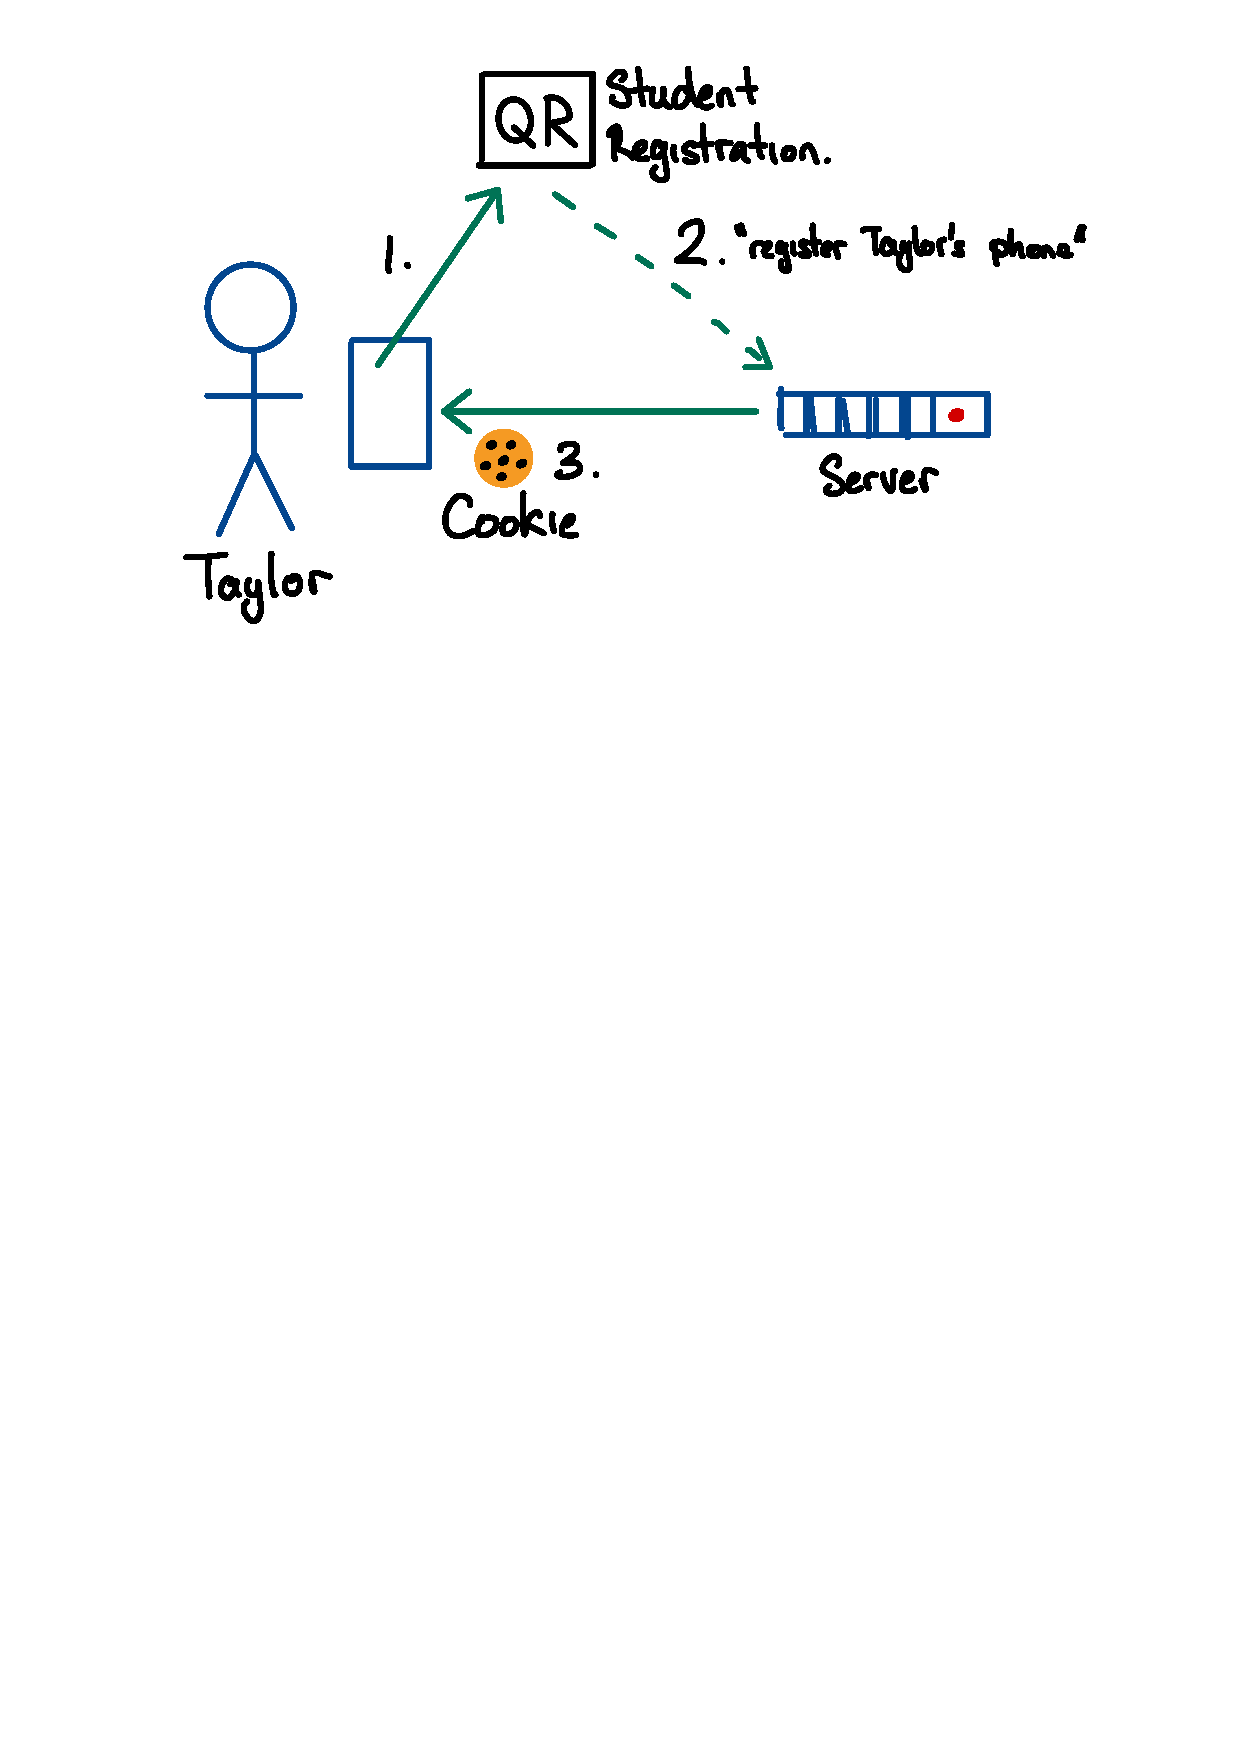
\includegraphics[scale=0.4]{figure/fig-student-registration.pdf}
\end{center}

\begin{enumerate}
\item The student (here, Taylor) uses their phone to scan their
      own personal \emph{student registration} QR code.

\item The student registration code directs the phone to the
      attendance server, which shows a page to register the phone
      as belonging to this student.

\item The student clicks a button on the registration page,
      which makes the server provide a \emph{cookie} (a special code) that
      contains their Aikikai identification number. The phone stores
      this cookie, and will give a copy back to the server if later requested.
\end{enumerate}

Students should typically only need to perform this registration process once.
They may need to register again if they change phones, or if they instruct the
web browser on their phone to clear the cookies it is holding.

Your own personal registration QR code is provided on the previous page.
If you lose these printed notes then your instructor can download a new PDF version
from the attendance site.
\end{minipage}
\hspace{2em}
%-----------------------------------------------------------
\begin{minipage}[t]{\dimexpr0.5\linewidth-1em}
\vspace{2em}
\textbf{2. Class Registration}
\begin{center}
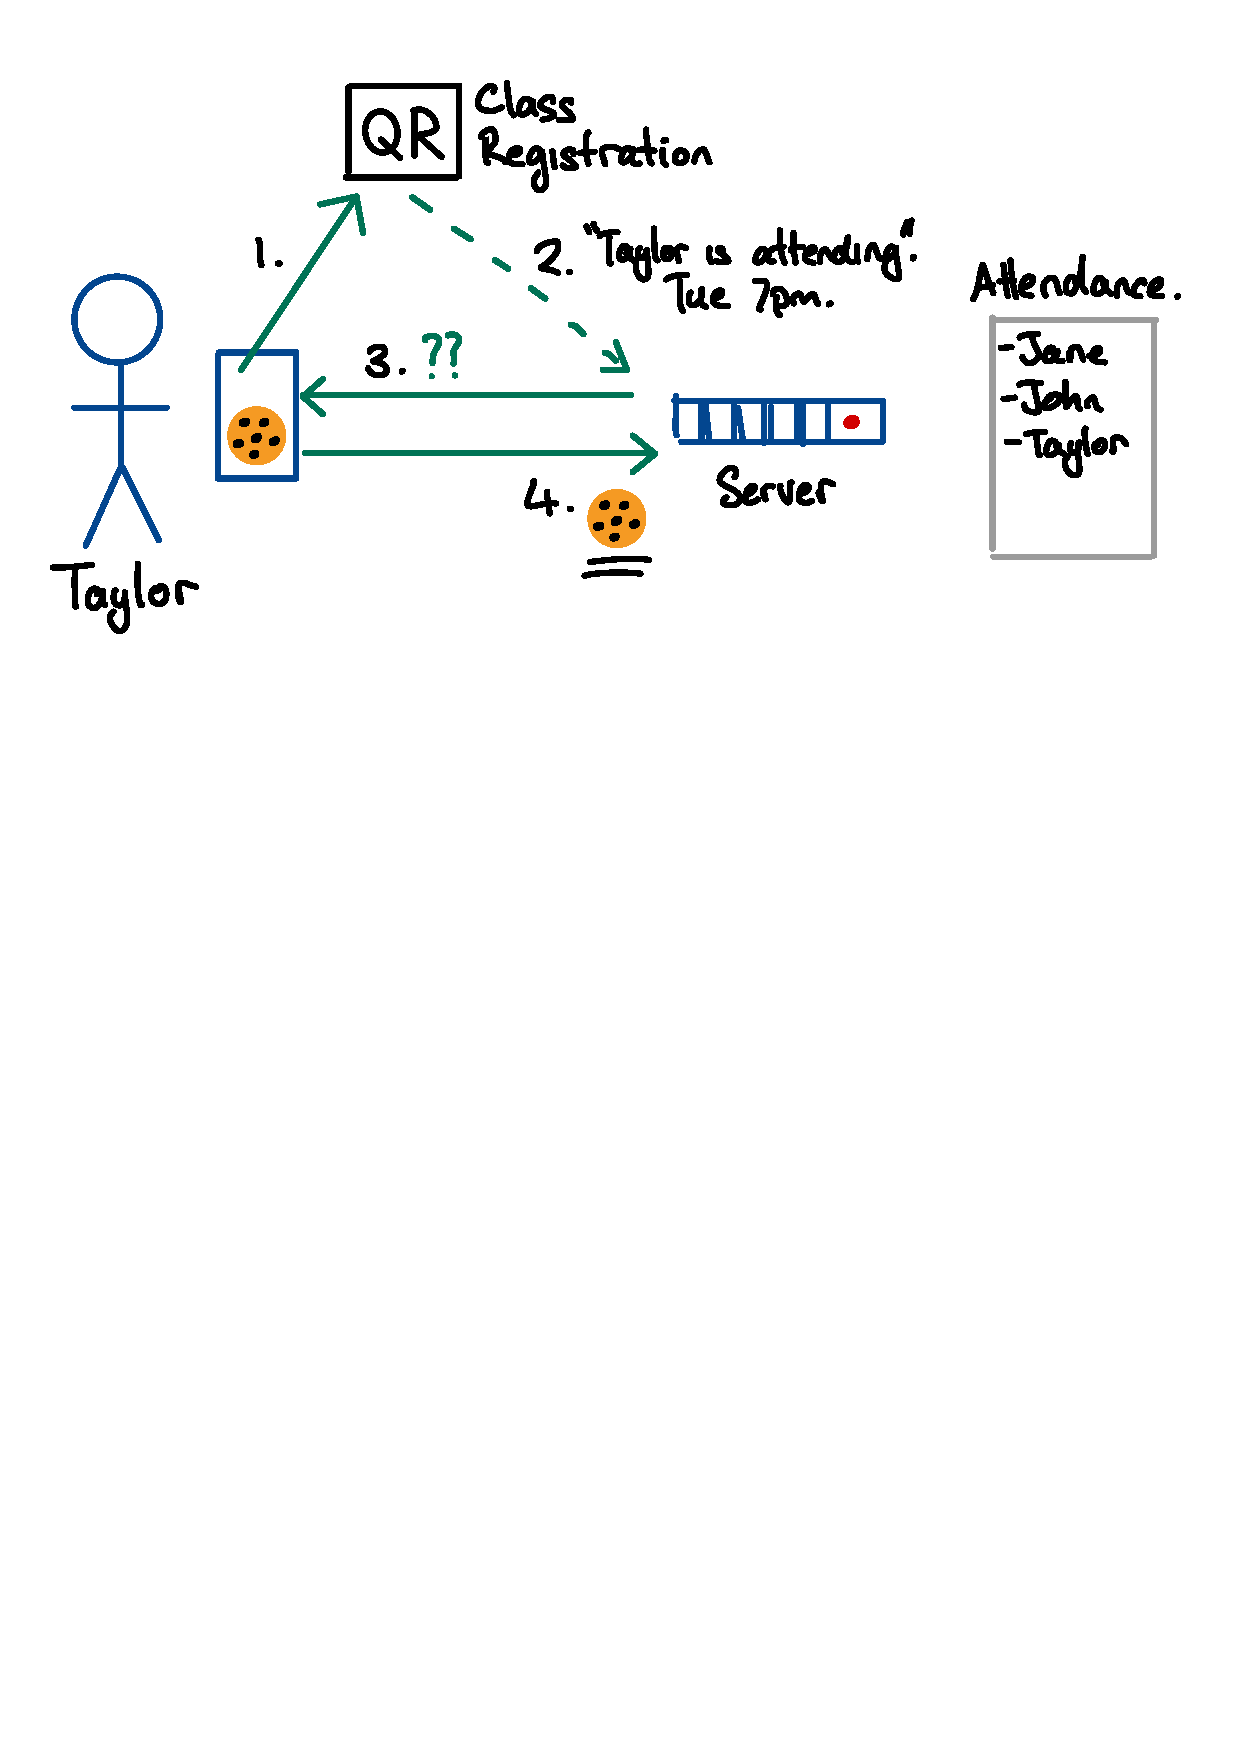
\includegraphics[scale=0.4]{figure/fig-class-registration.pdf}

\begin{enumerate}
\item When the student attends a class they use their phone to scan
      a different \emph{class registration} QR code.
\item The class registration code directs the phone back to the
      attendance server.
\item The server requests a copy of the cookie provided previously,
      which it uses to determine which student is connecting to it.
\item The shows a page which includes a button to add the
      student to the attendance list for the class.
\item The student clicks the button to have their name added to the list.
\end{enumerate}
\end{center}


\smallskip
%-----------------------------------------------------------
\textbf{3. Frequently Asked Questions}
\begin{enumerate}
\item \emph{Q: What if I don't have a phone, or don't bring it?}
      A: The class instructor can add your name to the attendance list
         directly, via a separate web page.

\item \emph{Q: Who has access to the attendance records?} \\
      A: Instructors and administrators that are part of Aikikai Australia.
         The physical computer that hosts the site is managed by a professional
         hosting company (Linode), located in Sydney, Australia. The hosting company
         also has access to the physical machine. The server does not run any other
         services besides the attendance system.

\item \emph{Q: Does clearing cookies from my phone affect my attendance records?}
      A: No. The cookie only contains your encoded Aikikai identification number.
         The cookie is used by the server to determine which student
         is connecting to it. The attendance records are stored on the server.

\item \emph{Q: What if I give my phone to someone else?} \\
      A: You can remove the cookie from your phone by either 1) using the ``clear cookies"
         functionality of your web browser, or 2) using the student registration QR code to return
         to the registration page and clicking ``unregister". You can unregister
         and re-register a phone whenever you like.
\end{enumerate}


\medskip
%-----------------------------------------------------------
\textbf{4. Contact Details}

Please contact Ben Lippmeier \texttt{benl@ouroborus.net} for
any questions, concerns or feedback.
This is a new system, so we are interested any bug reports or
ideas to make it easier to use.
\end{minipage}
